% Author: Izaak Neutelings (November 2020)
\documentclass[border=3pt,tikz]{standalone}
\usepackage{siunitx}
\usepackage{physics}
\usepackage{tikz}
\usepackage[outline]{contour} % glow around text
\usetikzlibrary{patterns,decorations.pathmorphing}
\usetikzlibrary{arrows.meta}
\tikzset{>=latex}
\contourlength{1.1pt}

\colorlet{mydarkblue}{blue!50!black}
\colorlet{myred}{red!65!black}
\colorlet{vcol}{green!45!black}
\colorlet{watercol}{blue!80!cyan!10!white}
\colorlet{darkwatercol}{blue!80!cyan!20!white}
\colorlet{metalcol}{blue!40!black!10!white}
\tikzstyle{force}=[->,myred,very thick,line cap=round]
\tikzstyle{vvec}=[->,very thick,vcol,line cap=round]
\tikzstyle{piston}=[blue!50!black,top color=blue!30,bottom color=blue!50,middle color=blue!20,shading angle=0]
\tikzstyle{water}=[draw=mydarkblue,top color=watercol!90,bottom color=watercol!90!black,shading angle=5]
\tikzstyle{vertical water}=[water,
  top color=watercol!90!black!90,bottom color=watercol!90!black!90,middle color=watercol!80,shading angle=90]
\tikzstyle{dark water}=[draw=mydarkblue,top color=darkwatercol,bottom color=darkwatercol!80!black,shading angle=5]
\tikzstyle{metal}=[draw=metalcol!20!black,top color=metalcol,bottom color=metalcol!90!black,shading angle=10]
\tikzstyle{width}=[{Latex[length=3,width=3]}-{Latex[length=3,width=3]}]
\def\tick#1#2{\draw[thick] (#1)++(#2:0.1) --++ (#2-180:0.2)}

\begin{document}


% PRESSURE
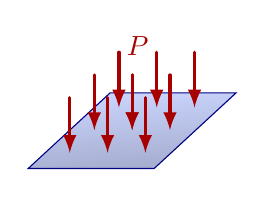
\begin{tikzpicture}[x={(1cm,0)},y={(0.65cm,0.6cm)},z={(0,1cm)}]
  \def\L{1.6} % cube side
  \def\P{0.7} % pressure size
  \draw[dark water] (0,0,0) -- (\L,0,0) -- (\L,\L,0) -- ( 0,\L,0) -- cycle;
  \draw[force] (0.5*\L,0.5*\L,1.01*\P) node[right=2,above=3] {$P$} --++ (0,0,-\P);
  \foreach \x/\y in {0.5/0.5,0.5/0.2,0.2/0.5,0.5/0.8,0.8/0.5,0.8/0.8,0.2/0.8,0.2/0.2,0.8/0.2}{
    \draw[force] (\x*\L,\y*\L,1.01*\P) --++ (0,0,-\P);
  }
\end{tikzpicture}


% PRESSURE DIRECTIONS - Pascal's principle
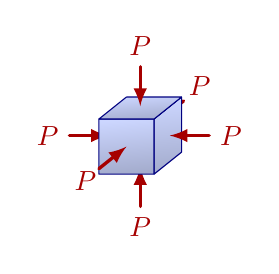
\begin{tikzpicture}[x={(1cm,0)},y={(0.5cm,0.4cm)},z={(0,1cm)}]
  \def\L{0.7} % cube side
  \def\P{0.5} % pressure size
  \draw[force] (\L/2,\L/2,-1.1*\P) node[below] {$P$} --++ (0,0,\P);
  \draw[force] (-1.1*\P,\L/2,\L/2) node[left] {$P$} --++ ( \P,0,0);
  \draw[force] (\L/2,\L+1.5*\P,\L/2) node[above right=-2] {$P$} --++ (0,-1.4*\P,0);
  \draw[dark water,rounded corners=0.1] (\L,0, 0) -- (\L,0,\L) -- (\L,\L,\L) -- (\L,\L, 0) -- cycle;
  \draw[dark water,rounded corners=0.1] ( 0,0, 0) -- ( 0,0,\L) -- (\L, 0,\L) -- (\L, 0, 0) -- cycle;
  \draw[dark water,rounded corners=0.1] ( 0,0,\L) -- (\L,0,\L) -- (\L,\L,\L) -- ( 0,\L,\L) -- cycle;
  \draw[force] (\L/2,\L/2,\L+1.05*\P) node[above] {$P$} --++ (0,0,-\P);
  \draw[force] (\L+1.05*\P,\L/2,\L/2) node[right] {$P$} --++ (-\P,0,0);
  \draw[force] (\L/2,-1.4*\P,\L/2) node[below left=-3] {$P$} --++ (0,1.4*\P,0);
\end{tikzpicture}


% WATER COLUMN WEIGHT
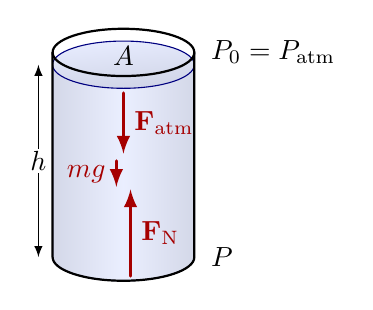
\begin{tikzpicture}
  \def\Rx{0.9}      % tank horizontal radius
  \def\Ry{0.3}      % tank vertical radius
  \def\H{2.6}       % height tank
  \def\h{0.94*\H}   % height water
  \def\y{0.40*\H}   % vertical position piece
  \def\F{0.45*\h}   % force
  
  % WATER
  \draw[vertical water]
    (-\Rx,\h) -- (-\Rx,0) arc (180:360:{\Rx} and {\Ry}) -- (\Rx,\h);
  \draw[water]
    (0,\h) ellipse ({\Rx} and {\Ry});
  
  % CONTAINER
  \draw[thick]
    (-\Rx,\H) -- (-\Rx,0) arc (180:360:{\Rx} and {\Ry}) -- (\Rx,\H);
  \draw[thick]
    (0,\H) ellipse ({\Rx} and {\Ry});
  
  % LABELS
  \draw[force] (-0.1*\Rx,\h/2) --++ (0,-0.3*\F) node[midway,left] {$mg$};
  \draw[force] (0.1*\Rx,-0.8*\Ry) --++ (0,\F) node[midway,right] {$\vb{F}_\mathrm{N}$};
  \draw[force] (0.0*\Rx,\h-1.2*\Ry) --++ (0,-0.7*\F) node[midway,right] {$\vb{F}_\mathrm{atm}$};
  \node[right] at (1.1*\Rx,\H) {$P_0=P_\mathrm{atm}$}; %{\contour{watercol}{$P_\mathrm{atm}$}};
  \node[right] at (1.1*\Rx,0) {$P$};
  \node[above=-4] at (0,\h) {$A$};
  \draw[<->] (-1.2*\Rx,0) --++ (0,\h) node[midway,fill=white,inner sep=1] {$h$};
  
\end{tikzpicture}


% WATER COLUMN WEIGHT
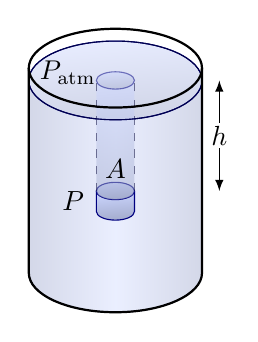
\begin{tikzpicture}
  \def\Rx{1.1}      % tank horizontal radius
  \def\Ry{0.5}      % tank vertical radius
  \def\rx{0.22*\Rx} % column horizontal radius
  \def\ry{0.22*\Ry} % column vertical radius
  \def\H{2.6}       % height tank
  \def\h{0.94*\H}   % height water
  \def\y{0.40*\H}   % vertical position piece
  \def\dy{0.10*\H}  % height piece
  
  % WATER
  \draw[vertical water]
    (-\Rx,\h) -- (-\Rx,0) arc (180:360:{\Rx} and {\Ry}) -- (\Rx,\h);
  \draw[water]
    (0,\h) ellipse ({\Rx} and {\Ry});
  
  % COLUMN + PIECE
  \draw[dark water]
    (-\rx,\y) -- (-\rx,\y-\dy) arc (180:360:{\rx} and {\ry}) -- (\rx,\y);
  \draw[dark water]
    (0,\y) ellipse ({\rx} and {\ry});
  \draw[dark water,opacity=0.50,draw=none] % column
    (-\rx,\h) -- (-\rx,\y) arc (180:360:{\rx} and {\ry}) -- (\rx,\h) arc(360:180:{\rx} and {\ry}) -- cycle;
  \draw[blue!20!black,dashed,very thin,opacity=0.50] (-\rx,\y) -- (-\rx,\h) (\rx,\y) -- (\rx,\h);
  \draw[dark water,opacity=0.50] % top column
    (0,\h) ellipse ({\rx} and {\ry});
  \draw[blue!30!black]
    (0,\h) ellipse ({\Rx} and {\Ry});
  
  % CONTAINER
  \draw[thick]
    (-\Rx,\H) -- (-\Rx,0) arc (180:360:{\Rx} and {\Ry}) -- (\Rx,\H);
  \draw[thick]
    (0,\H) ellipse ({\Rx} and {\Ry});
  
  % LABELS
  \node[scale=0.98] at ({-0.45*(\Rx+\rx)},1.04*\h) {$P_\mathrm{atm}$}; %{\contour{watercol}{$P_\mathrm{atm}$}};
  \node at ({-0.40*(\Rx+\rx)},{\y-0.5*\dy}) {$P$};
  \node[above=-2] at (0,\y+\ry) {$A$};
  \draw[<->] (1.2*\Rx,\y) --++ (0,\h-\y) node[midway,fill=white,inner sep=1] {$h$};
  
\end{tikzpicture}


% PRESSURE HEIGTH DIFFERENCE
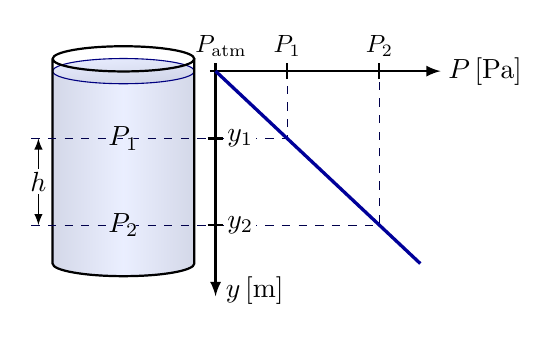
\begin{tikzpicture}
  \def\Rx{0.9}      % tank horizontal radius
  \def\Ry{0.16}     % tank vertical radius
  \def\H{2.6}       % height tank
  \def\h{0.94*\H}   % height water
  \def\ya{0.65*\h}  % vertical position A
  \def\yb{0.20*\h}  % vertical position B
  
  % WATER
  \draw[vertical water]
    (-\Rx,\h) -- (-\Rx,0) arc (180:360:{\Rx} and {\Ry}) -- (\Rx,\h);
  \draw[water]
    (0,\h) ellipse ({\Rx} and {\Ry});
  \draw[thick]
    (-\Rx,\H) -- (-\Rx,0) arc (180:360:{\Rx} and {\Ry}) -- (\Rx,\H)
    (0,\H) ellipse ({\Rx} and {\Ry});
  
  % LABELS
  %\node at ({-0.44*(\Rx+\rx)},1.04*\h) {$P_\mathrm{atm}$}; %{\contour{watercol}{$P_\mathrm{atm}$}};
  %\node at ({-0.40*(\Rx+\rx)},{\y-0.5*\dy}) {$P$};
  \draw[blue!30!black,dashed] (-1.3*\Rx,\ya) --++ (2.6*\Rx,0);
  \draw[blue!30!black,dashed] (-1.3*\Rx,\yb) --++ (2.6*\Rx,0);
  \draw[<->] (-1.2*\Rx,\yb) --++ (0,\ya-\yb) node[midway,fill=white,inner sep=1] {$h$};
  \node at (0,\ya) {\contour{watercol!80}{$P_1$}};
  \node at (0,\yb) {\contour{watercol!80}{$P_2$}};
  
  % AXIS
  \begin{scope}[shift={(1.3*\Rx,0)}]
    \draw[->,thick] (-0.03*\h,\h) --++ (1.2*\h,0) node[right=-1] {$P$\,[Pa]};
    \draw[->,thick] (0,1.03*\h) --++ (0,-1.2*\h) node[above=2,right] {$y$\,[m]};
    \draw[blue!30!black,dashed] (0,\ya) -| ({\H-\H/(\h)*\ya},\h);
    \draw[blue!30!black,dashed] (0,\yb) -| ({\H-\H/(\h)*\yb},\h);
    \tick{0,\ya}{180} node[right=0,fill=white,inner sep=1] {$y_1$};
    \tick{0,\yb}{180} node[right=0,fill=white,inner sep=1] {$y_2$};
    %\tick{0,\h}{180}; %node[above=2,right=-1] {$h$};
    \tick{0,\h}{-90} node[right=2,above=-1,scale=0.9] {$P_\mathrm{atm}$};
    \tick{{\H-\H/(\h)*\ya},\h}{-90} node[above=-1,scale=0.9] {$P_1$};
    \tick{{\H-\H/(\h)*\yb},\h}{-90} node[above=-1,scale=0.9] {$P_2$};
    %\tick{0.8*\H,0}{90} node[below=-1,scale=0.9] {$P_\mathrm{atm}+\rho g H$};
    \draw[blue!60!black,very thick] (0,\h) -- (\H,0);
  \end{scope}
  
\end{tikzpicture}


% PRESSURE HEIGTH DIFFERENCE
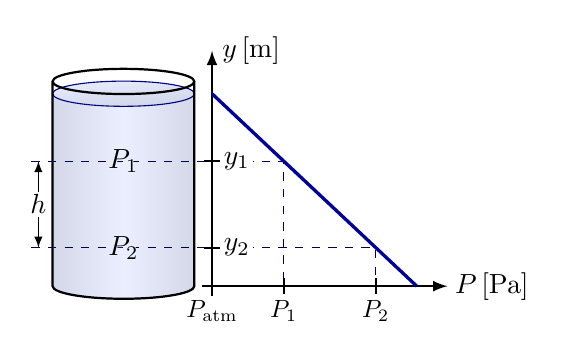
\begin{tikzpicture}
  \def\Rx{0.9}      % tank horizontal radius
  \def\Ry{0.16}     % tank vertical radius
  \def\H{2.6}       % height tank
  \def\h{0.94*\H}   % height water
  \def\ya{0.65*\h}  % vertical position A
  \def\yb{0.20*\h}  % vertical position B
  
  % WATER
  \draw[vertical water]
    (-\Rx,\h) -- (-\Rx,0) arc (180:360:{\Rx} and {\Ry}) -- (\Rx,\h);
  \draw[water]
    (0,\h) ellipse ({\Rx} and {\Ry});
  \draw[thick]
    (-\Rx,\H) -- (-\Rx,0) arc (180:360:{\Rx} and {\Ry}) -- (\Rx,\H)
    (0,\H) ellipse ({\Rx} and {\Ry});
  
  % LABELS
  %\node at ({-0.44*(\Rx+\rx)},1.04*\h) {$P_\mathrm{atm}$}; %{\contour{watercol}{$P_\mathrm{atm}$}};
  %\node at ({-0.40*(\Rx+\rx)},{\y-0.5*\dy}) {$P$};
  \draw[blue!30!black,dashed] (-1.3*\Rx,\ya) --++ (2.6*\Rx,0);
  \draw[blue!30!black,dashed] (-1.3*\Rx,\yb) --++ (2.6*\Rx,0);
  \draw[<->] (-1.2*\Rx,\yb) --++ (0,\ya-\yb) node[midway,fill=white,inner sep=1] {$h$};
  \node at (0,\ya) {\contour{watercol!80}{$P_1$}};
  \node at (0,\yb) {\contour{watercol!80}{$P_2$}};
  
  % AXIS
  \begin{scope}[shift={(1.25*\Rx,0)}]
    \draw[->,thick] (-0.05*\H,0) --++ (1.2*\H,0) node[right=-1] {$P$\,[Pa]};
    \draw[->,thick] (0,-0.05*\H) --++ (0,1.2*\H) node[right] {$y$\,[m]};
    \draw[blue!30!black,dashed] (0,\ya) -| ({\H-\H/(\h)*\ya},0);
    \draw[blue!30!black,dashed] (0,\yb) -| ({\H-\H/(\h)*\yb},0);
    \tick{0,\ya}{180} node[right=0,fill=white,inner sep=1] {$y_1$};
    \tick{0,\yb}{180} node[right=0,fill=white,inner sep=1] {$y_2$};
    %\tick{0,\h}{180}; %node[above=2,right=-1] {$h$};
    \tick{0,0}{90} node[below=-1,scale=0.9] {$P_\mathrm{atm}$};
    \tick{{\H-\H/(\h)*\ya},0}{90} node[below=-1,scale=0.9] {$P_1$};
    \tick{{\H-\H/(\h)*\yb},0}{90} node[below=-1,scale=0.9] {$P_2$};
    %\tick{0.8*\H,0}{90} node[below=-1,scale=0.9] {$P_\mathrm{atm}+\rho g H$};
    \draw[blue!60!black,very thick] (0,\h) -- (\H,0);
  \end{scope}
  
\end{tikzpicture}


% TORRICELLI
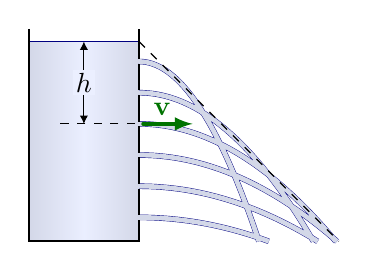
\begin{tikzpicture}
  \def\W{1.4}       % tank width
  \def\H{2.7}       % height tank
  \def\h{0.94*\H}   % height water
  \def\t{0.06}      % hole size
  \def\ya{0.12*\h}  % lowest hole
  \def\yb{0.90*\h}  % highest hole
  \def\ym{{\ya+3*(\yb-\ya)/(\N-1)}} % indicated hole
  \def\N{6}         % number of holes
  
  % WATER
  \draw[vertical water,draw=none]
    (-\W,0) rectangle++ (\W,\h);
  \draw[mydarkblue] (-\W,\h) --++ (\W,0);
  \draw[double=watercol!90!black!90,mydarkblue,double distance=1.7,line width=0.15]
  \foreach \i [evaluate={\y=\ya+(\i-1)*(\yb-\ya)/(\N-1);}] in {1,...,\N}{ %;\v=1.2*sqrt(\h-\y)
      plot[samples=100,smooth,variable=\x,domain=0:2*sqrt(\y*(\h-\y))](\x,{\y-\x*\x/4/(\h-\y)})
  };
  \draw[dashed] (0,\h) -- (\h,0);
  \draw[dashed] (-0.05,\ym) --++ (-0.75*\W,0);
  \draw[width]
    (-0.5*\W,\h) -- (-0.5*\W,\ym)
    node[midway,fill=watercol!80,inner sep=1] {$h$};
  \draw[vvec] (0.05,\ym) --++ (0.45*\W,0) node[midway,left=2,above=-1] {$\vb{v}$}; %_0
  
  % CONTAINER
  \draw[thick]
    (-\W,\H) |-++ (\W,-\H)
    \foreach \i [evaluate={\y=\ya+(\i-1)*(\yb-\ya)/(\N-1)}] in {1,...,\N}{
      -- (0,\y-\t/2) (0,\y+\t/2)
    } -- (0,\H);
  
\end{tikzpicture}


% PRESSURE HEIGTH DIFFERENCE
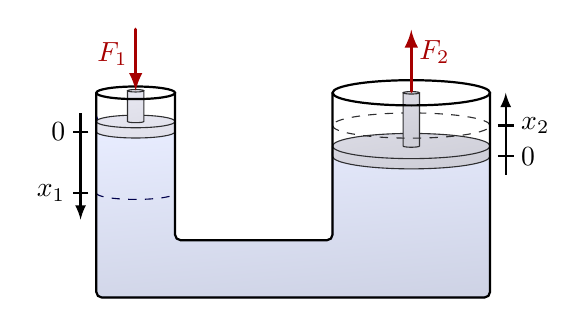
\begin{tikzpicture}
  \def\L{3.5}        % distance pistons
  \def\Lx{0.50}      % left piston horizontal radius
  \def\Ly{0.08}      % left piston vertical radius
  \def\Rx{1.00}      % right piston horizontal radius
  \def\Ry{0.16}      % right piston vertical radius
  \def\H{2.6}        % height tank
  \def\d{0.28*\H}    % diameter connecting pipe
  \def\hL{0.86*\H}   % left height water
  \def\hR{0.74*\H}   % right height water
  \def\pt{0.05*\H}   % piston thickness
  \def\prx{0.040*\H} % piston pole radius
  \def\pry{0.006*\H} % piston pole radius
  \def\pLl{0.15*\H}  % left piston pole length
  \def\pRl{0.26*\H}  % right piston pole length
  \def\xL{0.30*\H}   % right piston displacement
  \def\xR{\xL*\Lx/\Rx} % left piston displacement
  \def\F{0.3*\H}     % force magnitude
  
  % WATER
  \draw[water,rounded corners=2]
    (-\Lx,\hL) |-++ (\L+\Lx+\Rx,-\hL) |-++ (-2*\Rx,\hR) |-++ %arc (360:180:{\Rx} and {\Ry}) --++
    (-\L+\Lx+\Rx,-\hR+\d) |- cycle; %(-2*\Lx,\hL-\t) -- arc (360:180:{\Lx} and {\Ly}) -- cycle;
  \draw[blue!30!black,dashed,thin] (-\Lx,\hL-\pt-\xL) arc(180:360:{\Lx} and {\Ly});
  
  % PISTON
  \draw[metal]
    (-\Lx,\hL) --++ (0,-\pt) arc (180:360:{\Lx} and {\Ly}) --++ (0,\pt)
    (\L-\Rx,\hR) --++ (0,-\pt) arc (180:360:{\Rx} and {\Ry}) --++ (0,\pt)
    (0,\hL) ellipse ({\Lx} and {\Ly})
    (\L,\hR) ellipse ({\Rx} and {\Ry});
  \draw[metalcol!20!black,dashed,thin]
    (\L+\Rx,\hR-\pt+\xR) arc(0:180:{\Rx} and {\Ry});
  \draw[metal]
    (-\prx,\hL+\pLl) --++ (0,-\pLl) arc (180:360:{\prx} and {\pry}) --++ (0,\pLl)
    (\L-\prx,\hR+\pRl) --++ (0,-\pRl) arc (180:360:{\prx} and {\pry}) --++ (0,\pRl)
    (0,\hL+\pLl) ellipse ({\prx} and {\pry})
    (\L,\hR+\pRl) ellipse ({\prx} and {\pry});
  \draw[metalcol!20!black,dashed,thin]
    (\L-\Rx,\hR-\pt+\xR) arc(180:360:{\Rx} and {\Ry});
  
  % CONTAINER
  \draw[thick,rounded corners=2]
    (-\Lx,\H) |-++ (\L+\Lx+\Rx,-\H) --++ (0,\H)
    (\Lx,\H) |-++ (\L-\Lx-\Rx,-\H+\d) --++ (0,\H-\d);
  \draw[thick]
    (0,\H) ellipse ({\Lx} and {\Ly}) (\L,\H) ellipse ({\Rx} and {\Ry});
  
  % FORCES
  \draw[force] (0,\hL+\pLl+\F) --++ (0,-\F) node[pos=0.4,left=-1] {$F_1$};
  \draw[force] (\L,\hR+\pRl+0.02) --++ (0,\F) node[midway,above=3,right=-1] {$F_2$};
  
  % AXIS
  \draw[->,thick] (-\Lx-0.2*\Rx,0.9*\H) --++ (0,-0.52*\H); %node[left] {$x_1$};
  \draw[->,thick] (\L+1.2*\Rx,0.6*\H) --++ (0,0.40*\H); %node[right] {$x_2$};
  \tick{-\Lx-0.2*\Rx,\hL-\pt}{0} node[left=-1] {$0$};
  \tick{-\Lx-0.2*\Rx,\hL-\pt-\xL}{0} node[left=-1] {$x_1$};
  \tick{\L+1.2*\Rx,\hR-\pt}{180} node[right=-1] {$0$};
  \tick{\L+1.2*\Rx,{\hR-\pt+\xR}}{180} node[right=-1] {$x_2$};
  
\end{tikzpicture}


\end{document}
